% !TEX program = xelatex

\documentclass[aspectratio=169,20pt]{beamer}
\usepackage{wrapfig}
\usepackage{xcolor}
\definecolor{applegreen}{rgb}{0.55, 0.71, 0.0}
\definecolor{deepgreen}{rgb}{0.0, 0.5, 0.0}
\graphicspath{ {./images/} }
\usetheme{ost}

\title{εικόνα - Challenge Project}
\subtitle{OST — Ostschweizer Fachhochschule}
\date{\today}
\author{Lukas Ribi, Dominik Castelberg, Pascal Christen}
\institute{DS1 - Thomas Bocek }

\begin{document}

\begin{frame}
	\titlepage
\end{frame}

\begin{frame}{Goal}{1. Introduction}
	\underline{Problem}: Often you need to resize, adjust quality, and convert on-demand:
	\vspace{1in}
	\begin{columns}[onlytextwidth,T]
		\begin{column}{.25\linewidth}
			\begin{itemize}
				\item{Responsive Websites}
				\item{Upload of an image}
			\end{itemize}
		\end{column}
		\begin{column}{.65\linewidth}
			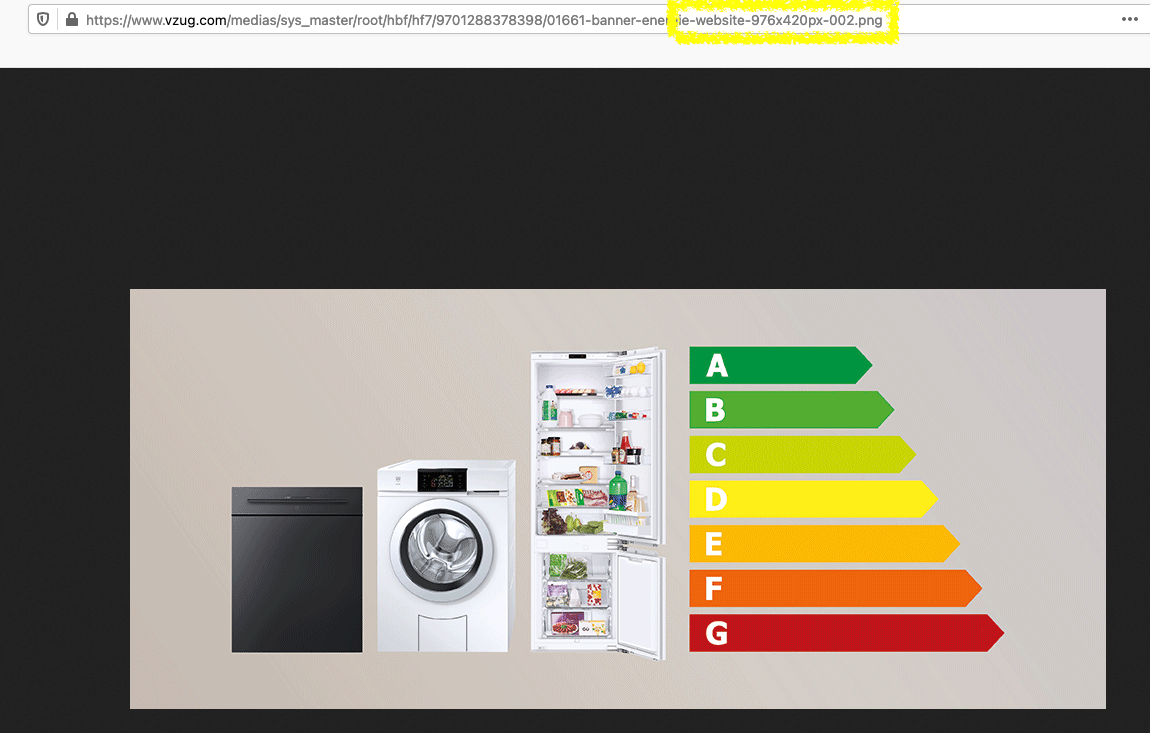
\includegraphics[scale=0.55]{vzug}
		\end{column}
	\end{columns}
	\underline{Solution}: Our \textit{eikona} service converts the image \textbf{on-the-fly} and provides a simple \textit{REST API}.
\end{frame}

\begin{frame}{Setup}{2. Technology}
	\begin{itemize}
		\item{Backend}
		\begin{itemize}
			\item{\href{https://golang.org/}{go} (1.16.3)}
			\begin{itemize}
				\item{\href{https://gin-gonic.com/}{gin} (1.7.1) with \href{https://github.com/dgraph-io/ristretto}{Ristretto} (0.0.3)}
				\item{JWT}
			\end{itemize}
		\end{itemize}
		\item{Frontend}
		\begin{itemize}
			\item{\href{https://reactjs.org/versions/}{ReactJS} (17.0.2)}
			\begin{itemize}
				\item{Material-UI}
				\item{Served by \href{https://nginx.org/}{Nginx} (1.20.0)}
			\end{itemize}
		\end{itemize}
		\item{Loadbalancer}
		\begin{itemize}
			\item{\href{https://traefik.io/}{Traefik} (2.4.8)}
		\end{itemize} 
		\item{Storage}
		\begin{itemize}
			\item{\href{https://www.postgresql.org/}{PostgreSQL} (13.2)}
			\item{\href{https://min.io/}{MinIO - Object Storage} (RELEASE.2021-03-26)}
		\end{itemize}
		\item{Presentation}
		\begin{itemize}
			\item{\href{https://github.com/ost-fh/Latex-Beamer-Theme}{LaTeX}}
		\end{itemize}       
	\end{itemize}
\end{frame}

\begin{frame}{System Diagram}{2. Technology}
	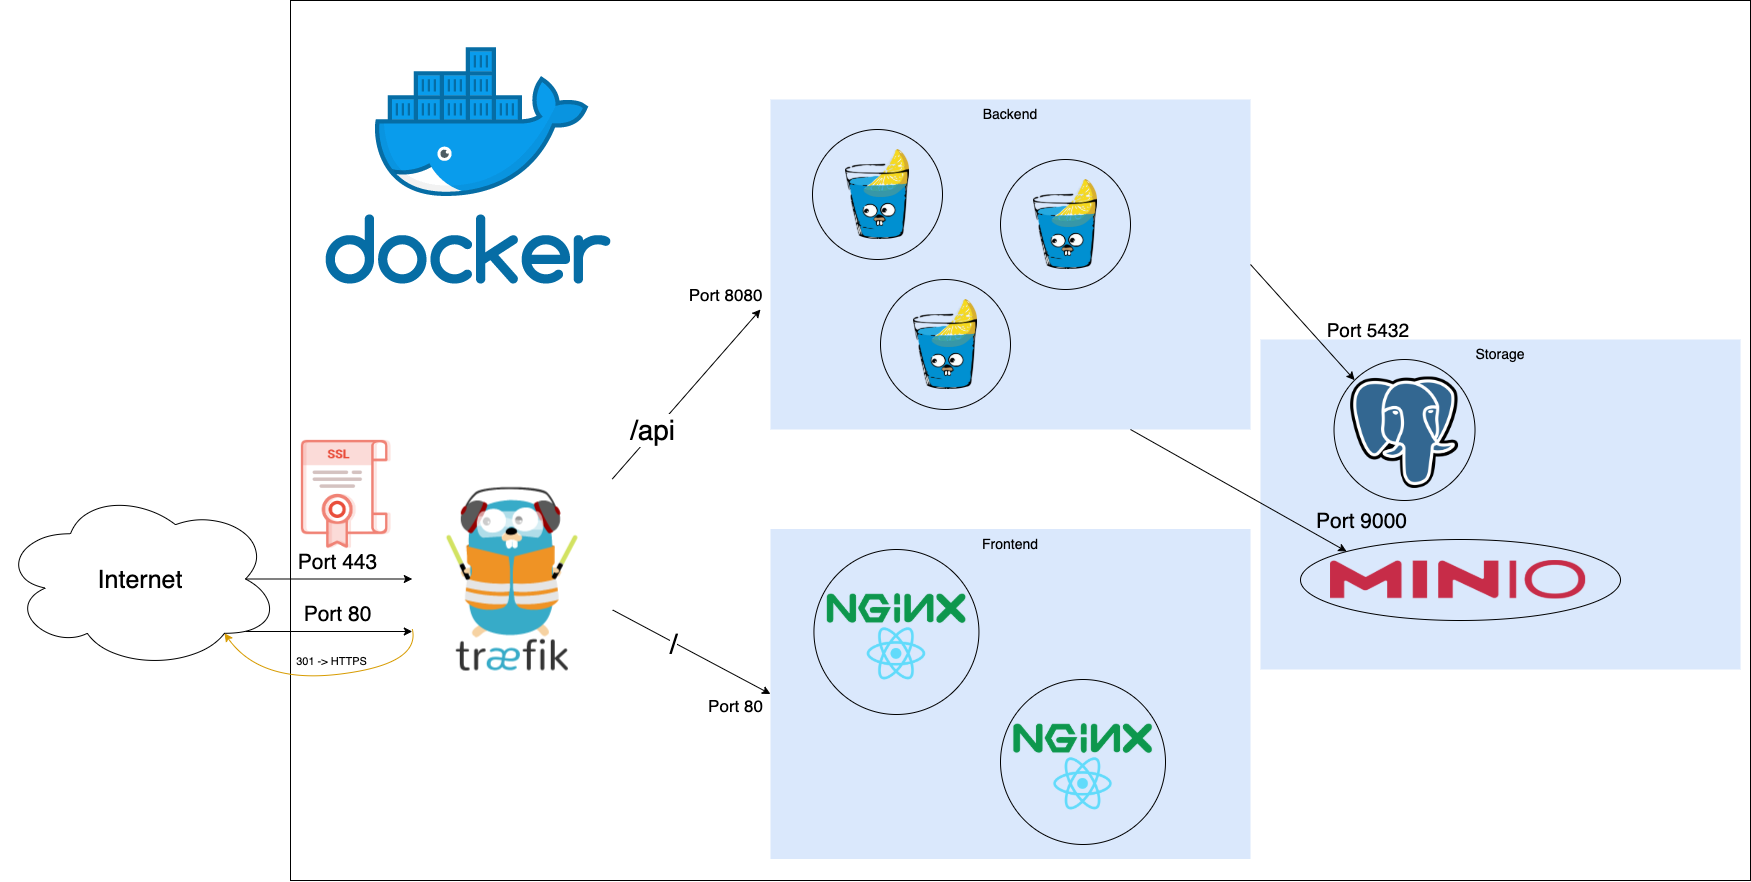
\includegraphics[scale=0.45]{Infrastruktur}	
\end{frame}

\begin{frame}{Data Model}{3. Development}
	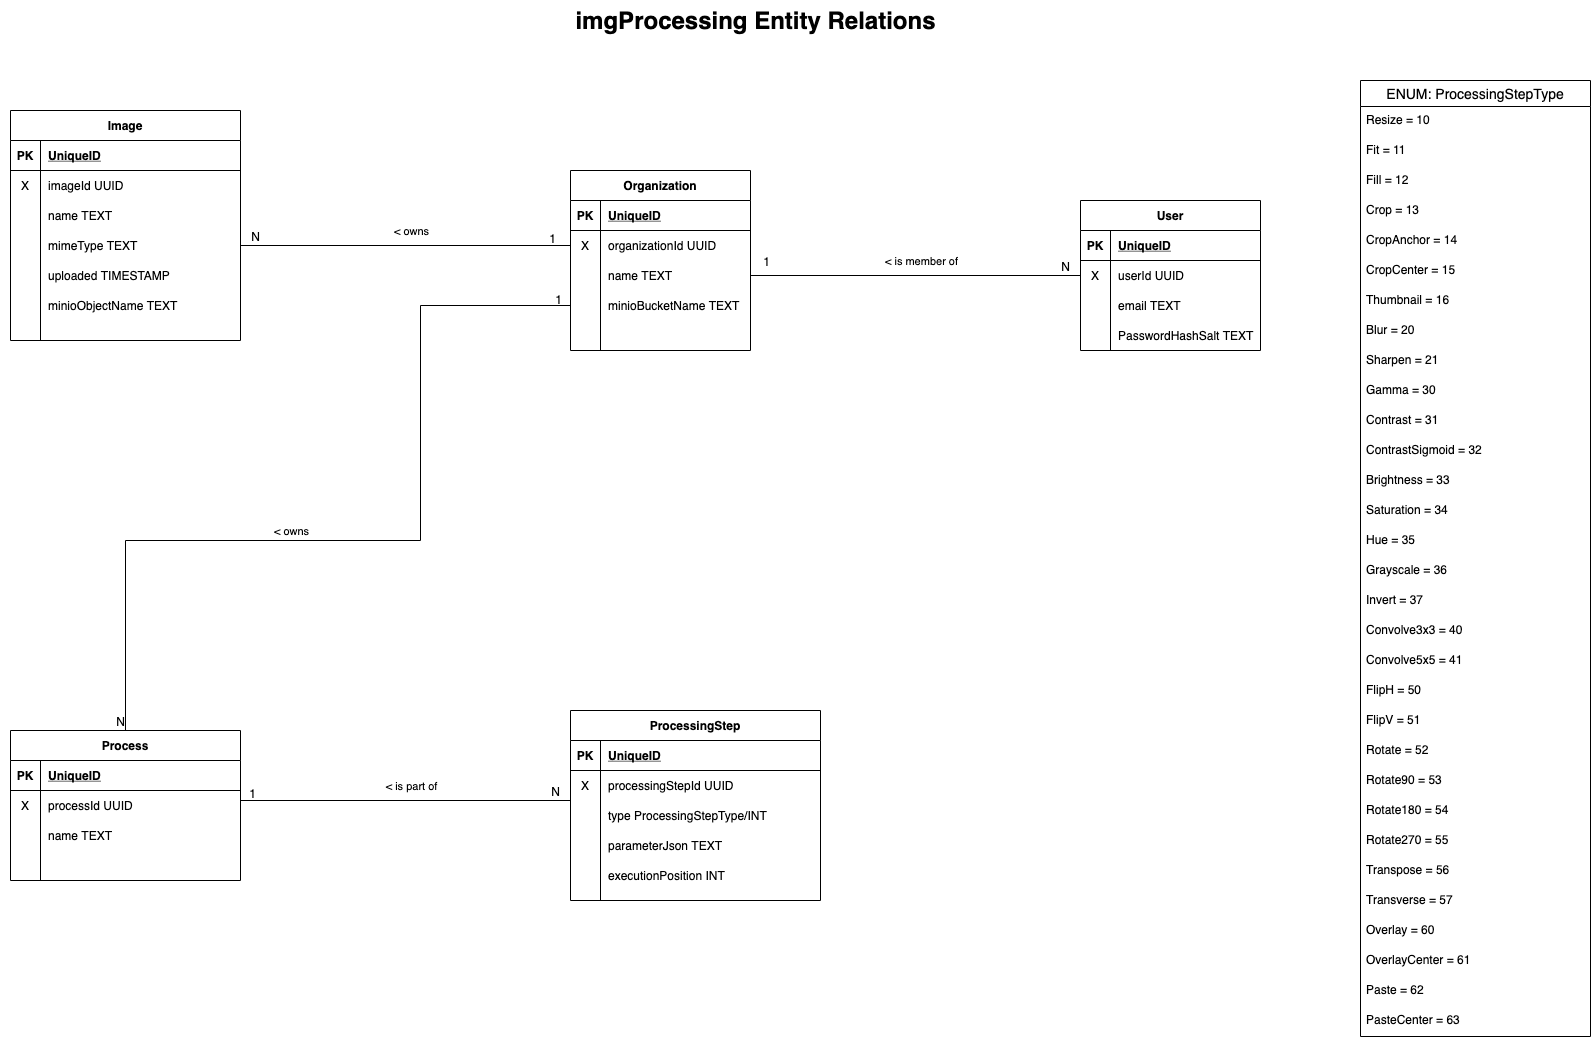
\includegraphics[scale=0.45]{db_model}
\end{frame}

\begin{frame}{Github Actions}{3. Development}
	\begin{itemize}
		\item{Docker Images - builded and versioned by Github Actions}
		\begin{itemize}
			\item{Frontend}
			\item{Backend}
		\end{itemize}
		\item{Security by scanning for \href{https://github.com/marketplace/actions/container-image-scan/}{CVE}}
		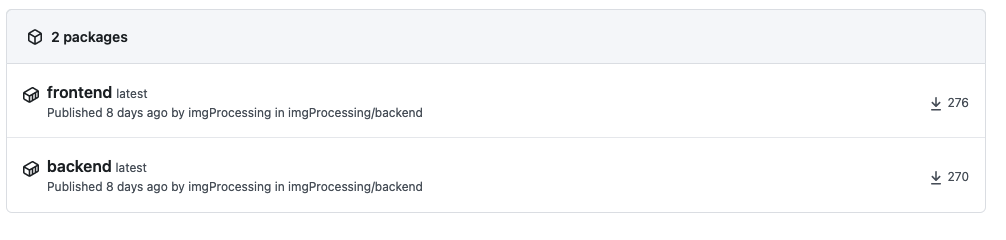
\includegraphics[scale=0.8]{action}
	\end{itemize}
\end{frame}

\begin{frame}{docker-compose}{3. Development}
	\begin{itemize}
		\item{Production and Development environment}
		\item{Restriced access on production}
		\item{Working with environments}
	\end{itemize}
\end{frame}

\begin{frame}{Loadbalancer}{3. Development}
	\underline{Traefik}:
	\begin{itemize}
		\item{Docker Socket mounted:}
		\begin{itemize}
			\item{+ Autodiscover}
			\item{- Security}
		\end{itemize}
		\item{HTTP -> HTTPS Middleware}
		\item{Self-signed cert with \href{https://github.com/FiloSottile/mkcert}{mkcert} for development}
		\item{Healthchecks}
	\end{itemize}
\end{frame}

\begin{frame}{Frontend}{3. Development}
	\begin{columns}[onlytextwidth,T]
		\begin{column}{.40\linewidth}
			\underline{ReactJS with Material-UI}:
			\vspace{1in}
			\begin{itemize}
				\item{Responsive design}
				\item{Simple error handling}
				\item{Functions:}
				\begin{itemize}
					\item{Dashboard}
					\item{Upload Image}
					\item{Create Process}
					\item{API Overview}
				\end{itemize}
			\end{itemize}
		\end{column}	
		\begin{column}{.60\linewidth}
			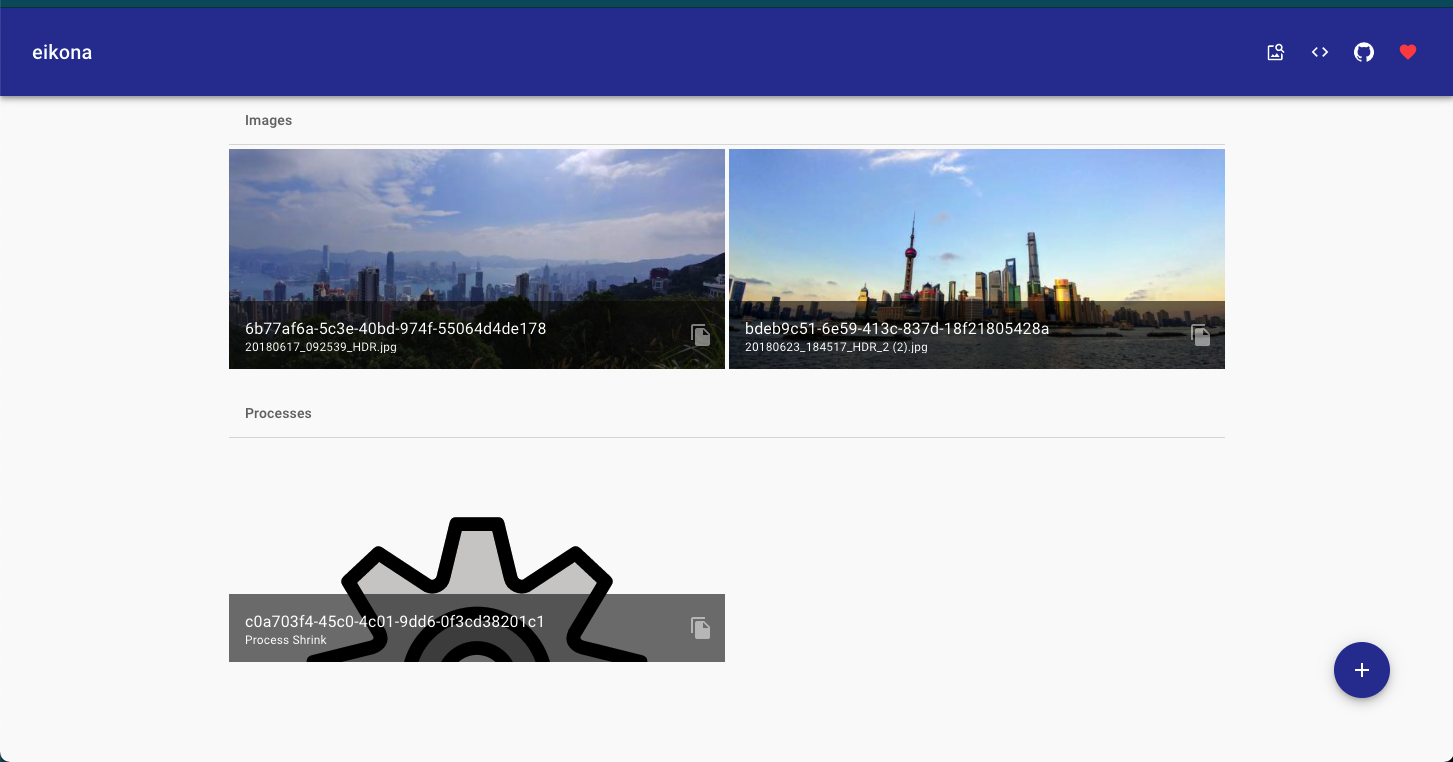
\includegraphics[scale=0.35]{frontend}
		\end{column}
	\end{columns}
\end{frame}

\begin{frame}{Backend}{3. Development}
	\underline{Golang}:
	\begin{itemize}
		\item{Image filtering using \href{https://github.com/disintegration/gift}{gift}:}
		\begin{itemize}
			\item{25 operations right now (expanding...)}
		\end{itemize}
		\item{REST API using \href{https://github.com/gin-gonic/gin}{gin}:}
		\begin{itemize}
			\item{JWT authentication using middleware}
			\item{API Documentation using \href{https://github.com/swaggo/swag}{swagger}}
		\end{itemize}
		\item{Quickwin: Simple caching at application level using \href{https://github.com/dgraph-io/ristretto}{Ristretto}}
		\begin{itemize}
			\item{TODO: Use varnish, nginx or traefik enterprise in front of application to handle image caching}
		\end{itemize}
	\end{itemize}
\end{frame}

\begin{frame}{Storage}{3. Development}
	\begin{columns}[onlytextwidth,T]
		\begin{column}{.40\linewidth}
			\underline{MinIO}:
			\vspace{1in}
			\begin{itemize}
				\item{High Performance, Kubernetes Native Object Storage}
				\item{Compatible with Amazon S3}
			\end{itemize}
		\end{column}
		\begin{column}{.60\linewidth}
			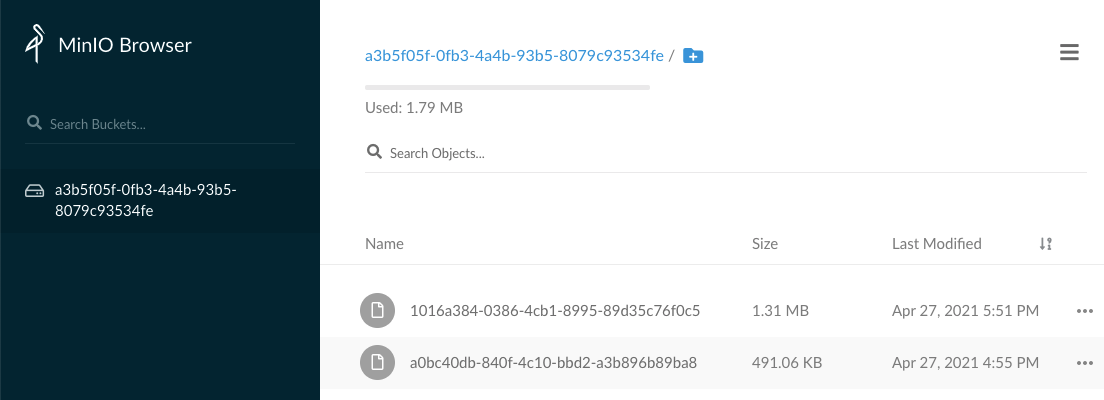
\includegraphics[scale=0.45]{minio}
		\end{column}
	\end{columns}
\end{frame}

\begin{frame}{Fulfillment of Requirements}{4. Legal}
	\begin{itemize}
		\item{Dockerized: \textcolor{deepgreen}{Used (images hosted on Github)}}
		\item{Load balancing: \textcolor{deepgreen}{Traefik}}
		\item{Scalable service: \textcolor{deepgreen}{Backend and Frontend}}
		\item{JWT Authentication: \textcolor{deepgreen}{Used}}
		\item{Latest FOSS: \textcolor{deepgreen}{Used}}
	\end{itemize}
\end{frame}

\begin{frame}{Demo}{}
	\href{https://eikona.pesc.xyz/}{https://eikona.pesc.xyz}
\end{frame}

\begin{frame}{End}{}
	\href{https://github.com/eikona-org/eikona}{Source Code}
\end{frame}

\end{document}